\documentclass[11pt]{article}

\usepackage[letterpaper,margin=0.82in]{geometry}
\usepackage[T1]{fontenc}
\usepackage{lmodern}
\usepackage{microtype}
\usepackage{graphicx}
\usepackage{booktabs}
\usepackage{tabularx}
\usepackage{array}
\usepackage{longtable}
\usepackage{multirow}
\usepackage{enumitem}
\usepackage{caption}
\usepackage{float}
\usepackage{placeins}
\usepackage{xcolor}
\usepackage{hyperref}
\usepackage{fancyhdr}
\usepackage{setspace}
\usepackage{amsmath}
\usepackage{amssymb}

\definecolor{navy}{HTML}{17365D}
\definecolor{slate}{HTML}{4E5D6C}
\definecolor{lightblue}{HTML}{EAF2F8}
\definecolor{lightgray}{HTML}{F3F4F6}
\hypersetup{
  colorlinks=true,
  linkcolor=navy,
  citecolor=navy,
  urlcolor=navy,
  pdftitle={Reconstructing a Transparent Cereal Capacity Index},
  pdfsubject={Concise revised solo Food Security course-project report}
}

\captionsetup{font=small,labelfont=bf}
\setlist[itemize]{leftmargin=1.35em,itemsep=2pt,topsep=3pt}
\setlist[enumerate]{leftmargin=1.55em,itemsep=2pt,topsep=3pt}
\setlength{\parindent}{0pt}
\setlength{\parskip}{5pt}
\setstretch{1.08}
\newcolumntype{Y}{>{\raggedright\arraybackslash}X}
\newcolumntype{L}[1]{>{\raggedright\arraybackslash}p{#1}}
\newcommand{\score}{\textit{Capacity Score v2}}
\newcommand{\rhoS}{\ensuremath{\rho_{S}}}
\newcommand{\NA}{---}

\pagestyle{fancy}
\fancyhf{}
\fancyhead[L]{\small Transparent Cereal Capacity Index}
\fancyhead[R]{\small Revised course-project report}
\fancyfoot[C]{\thepage}
\renewcommand{\headrulewidth}{0.3pt}

\begin{document}

\begin{titlepage}
\thispagestyle{empty}
\vspace*{0.85in}
{\color{navy}\rule{\textwidth}{1.5pt}}\\[0.35in]
{\Huge\bfseries Reconstructing a Transparent\\[0.10in]
Cereal Capacity Index\par}
\vspace{0.18in}
{\LARGE A 30-Country Food Security Case Study\par}
\vspace{0.32in}
{\color{navy}\rule{\textwidth}{0.7pt}}\\[0.45in]

{\large Concise revised technical report\par}
\vspace{0.18in}
{\large MGT 6203 course-project reconstruction\par}

\vfill
\begin{minipage}{0.92\textwidth}
\small
\textbf{Status and ownership.} Public portfolio release, reconstructed on 29 August 2026 from a sole-author course project. The repository owner independently completed the original project end to end, including research framing, data collection and preprocessing, index design, modeling, interpretation, visualization, and reporting.

\textbf{Scope.} This report describes a transparent country-level cereal supply/trade capacity index and an audit of its associations. It does not claim to forecast hunger, measure household food access, or identify causal effects.
\end{minipage}
\vspace{0.35in}
\end{titlepage}

\pagenumbering{roman}

\section*{Executive Summary}
\addcontentsline{toc}{section}{Executive Summary}

This reconstruction answers a narrower and more defensible question than the original 154-page report: \emph{can official data support a transparent ranking of national cereal supply and trade capacity, and what can cautious explanatory analysis reveal about that constructed score?}

The revised project keeps the useful core of the earlier work---manual index design, expert constraints, country comparison, linear interpretation, and one nonlinear model---while removing the notebook-like accumulation of t-SNE, multiple tree libraries, unrestricted SHAP dependence plots, and Category-specific ICE/PDP plots. It also replaces a synthetic annual Global Hunger Index (GHI) component with two directly observable capacity components:

\[
\score_{c,t}=0.50\,R(\mathrm{SSR}_{c,t})+0.50\,R(\mathrm{CerealProductionPerPerson}_{c,t}),
\]

where each $R(\cdot)$ is a within-year percentile rank from 0 to 1 and SSR is derived from FAOSTAT Food Balances production, import, and export quantities. The score covers 30 countries from 2010--2023. Japan remains in the Legacy archive but is not imputed into v2 because the FAOSTAT Food Balances cereal series is absent for Japan in this window.

\textbf{What held up.}

\begin{itemize}
  \item The old three-component weight search was exactly reproduced as a deterministic 1\% simplex grid, not a Monte Carlo simulation. The reported 19/15/66 weights are the first of three tied minimum-TV solutions under the original traversal rule.
  \item The v2 country ordering is insensitive to reasonable weight and normalization choices: the 50/50 and 56/44 rankings correlate at \rhoS=0.998, and rank versus annual min--max normalization correlates at \rhoS=0.989.
  \item The original expert labels remain useful comparison slices, but they do not define v2. No value among 101 SSR weights satisfies all four old category-ordering hypotheses.
  \item A country-grouped shallow random forest lowers pooled out-of-fold MAE from 0.230 to 0.192 and RMSE from 0.277 to 0.229. However, only two of five held-out-country folds have positive $R^2$, so this is limited, heterogeneous structural explanation rather than strong prediction.
  \item Arable land per person is the only predictor with positive held-out permutation importance in all five folds. Other visually consistent SHAP patterns add little or inconsistent held-out information and are therefore demoted to the appendix.
  \item Higher v2 scores are directionally associated with lower official prevalence of undernourishment (PoU; \rhoS=-0.31) and lower moderate-or-severe food insecurity experience (FIES; \rhoS=-0.27). These modest correlations support directional coherence, not validation as a hunger or household-access measure.
\end{itemize}

\textbf{Bottom line.} The revised project is defensible as a reproducible, interpretable composite-index case study. Its strongest contribution is not forecasting. It is the explicit separation of (i) a narrow capacity construct, (ii) expert hypotheses that may be contradicted, (iii) exploratory country structure, (iv) country-grouped attribution, and (v) external outcomes that remain outside the index.

\newpage
\begin{abstract}
The original course project combined two constructed supply indicators with an annually interpolated Global Hunger Index, calibrated weights to expert category orderings, and used numerous linear, tree, and post-hoc explanation methods. This revision narrows the target to national cereal supply/trade capacity and rebuilds the analysis from preserved official-source snapshots. Capacity Score v2 combines annual percentile ranks of an SSR derived from FAOSTAT Food Balances and World Bank cereal production per person for 30 countries in 2010--2023. Weight, normalization, and temporal diagnostics show high rank robustness, while none of 101 weights reproduces all four Legacy category orderings. On six prespecified, non-component World Development Indicators over 2010--2021, Ward clustering yields an exploratory four-cluster cut dominated in part by extreme country profiles. Five-fold country-grouped evaluation gives pooled out-of-fold $R^2=-0.231$ for ordinary least squares and $R^2=0.319$ for a fixed shallow random forest, with substantial fold heterogeneity. Arable land per person is the only feature with positive held-out permutation importance in every fold. Country-median v2 scores have modest inverse rank associations with official PoU and FIES. The reconstruction therefore supports a transparent descriptive capacity index and cautious model attribution, but not a forecast, causal model, or comprehensive measure of food security.
\end{abstract}

\textbf{Keywords:} composite index; cereal self-sufficiency; food security; grouped validation; interpretable machine learning; construct alignment

\tableofcontents
\clearpage
\pagenumbering{arabic}

\section{Revision Question and Analytical Boundary}

Food security includes availability, access, utilization, and stability. A country can produce or import substantial cereal supplies while still experiencing household-level deprivation; conversely, a country with limited domestic production may secure access through trade and income. The revised project therefore does not label its score a complete food-security index. It asks a narrower question about \emph{national cereal supply/trade capacity}.

This distinction repairs the main conceptual weakness of the earlier report. The Legacy composite mixed a constructed self-sufficiency ratio, cereal production per person, and an inverted GHI series. GHI was available only at selected reference points but was converted into an annual series through interpolation, endpoint filling, and synthetic values for several high-income countries. It then received 66\% of the final weight. As a result, the Legacy score blended productive capacity with a hunger outcome and could appear externally aligned with hunger partly by construction.

The revised design separates five questions:

\begin{enumerate}
  \item Can two official cereal-capacity components generate a transparent, stable country ordering?
  \item Which preserved expert orderings are supported or contradicted without calibrating weights to force agreement?
  \item What country profiles appear in a small, prespecified set of contextual indicators?
  \item Which contextual indicators are associated with the constructed score when whole countries are held out?
  \item Is the capacity ranking directionally aligned with PoU and FIES, which remain external outcomes?
\end{enumerate}

The study unit is a country-year. No result should be transferred to households or individuals. Model outputs are associations with a constructed rank target, not estimates of interventions. The earlier time-forward PoU experiment, which failed to beat a persistence baseline, is preserved as a negative result rather than hidden or repaired with a larger model.

\begin{figure}[H]
\centering
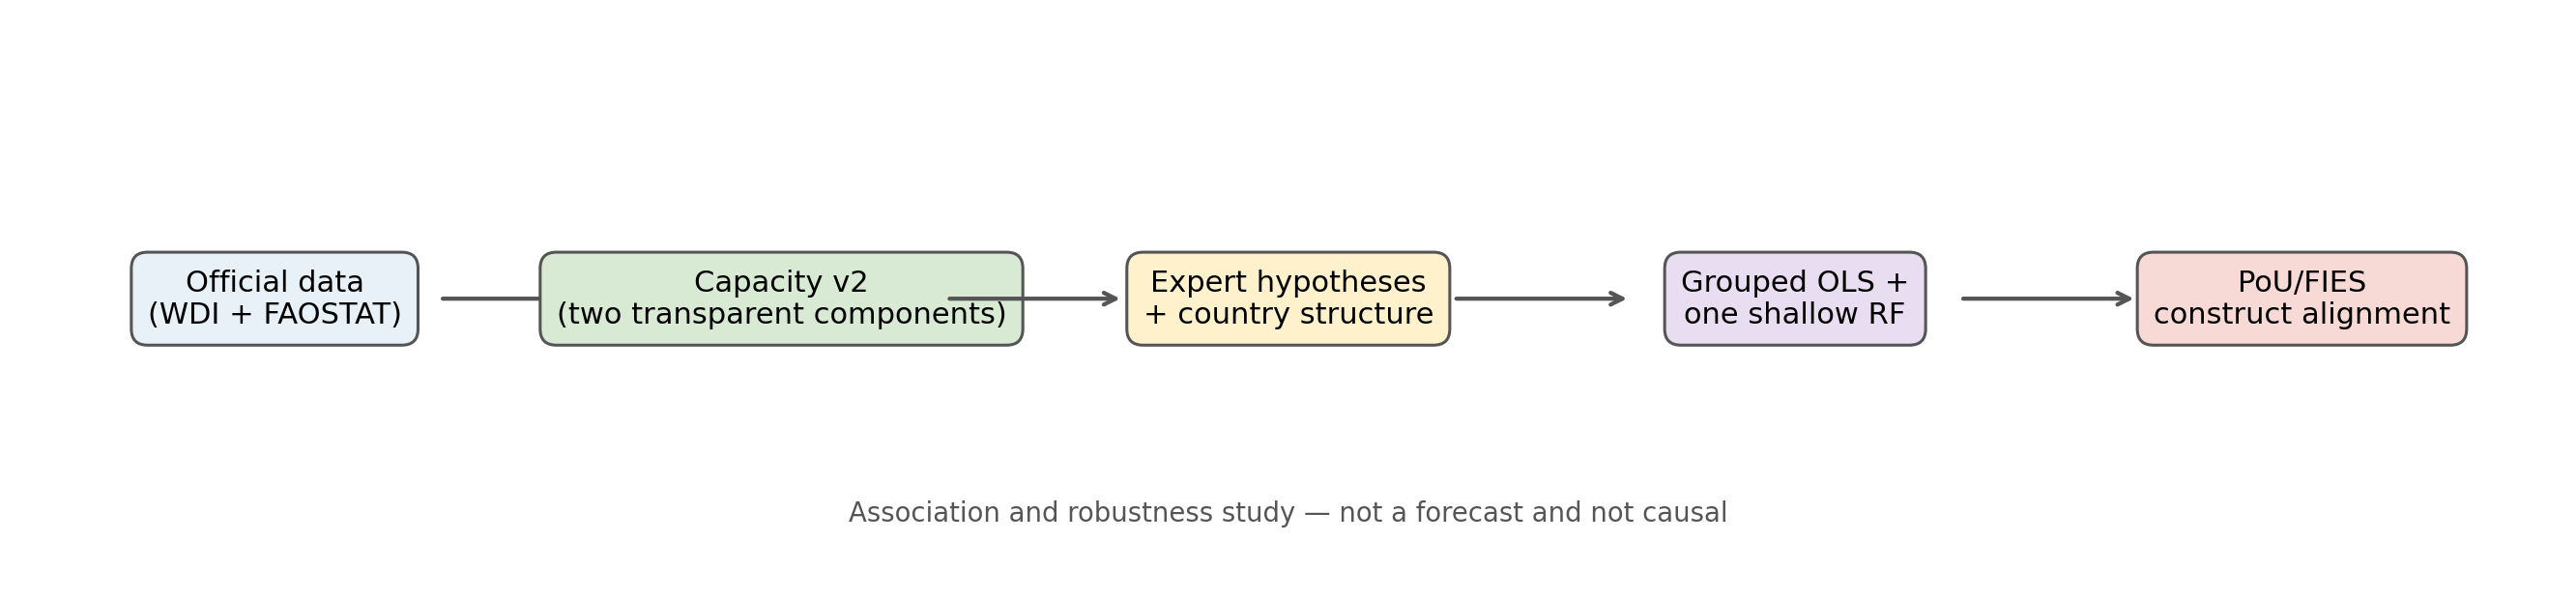
\includegraphics[width=0.92\textwidth]{../figures/method_flow.png}
\caption{Revised analytical flow. Hunger and food-access outcomes are kept outside the capacity index and used only for descriptive alignment.}
\label{fig:flow}
\end{figure}

\section{Data and Construct Definition}

\subsection{Sources, coverage, and semantics}

The reconstruction uses archived snapshots rather than undocumented spreadsheet copies. World Bank indicators were obtained through the v2 Indicator API, with query URLs, access timestamps, metadata, WDI update date, and SHA-256 hashes preserved. The six explanatory indicators form a complete grid of 31 countries $\times$ 12 years $\times$ six series (2,232 values); the 30-country v2 modeling panel therefore requires no imputation. The World Bank API is designed for programmatic access to indicator and country-time queries \cite{worldbankapi,worldbankqueries}.

FAOSTAT Food Balances provide annual production, imports, and exports for ``Cereals - Excluding Beer.'' The cereal self-sufficiency ratio (SSR) is transparently derived as production divided by domestic availability, consistent with the standard supply-utilization definition \cite{faohandbook,faofbs}. PoU and FIES are official three-year-average food-security indicators \cite{faohunger}; censoring and publication status are preserved rather than converted into ordinary missing values.

\begin{table}[H]
\centering
\caption{Data sources, semantics, coverage, and analytical roles.}
\label{tab:data}
\scriptsize
\begin{tabularx}{\textwidth}{L{2.45cm} L{3.45cm} L{2.45cm} L{4.20cm} Y}
\toprule
Source/code & Definition and unit & Coverage & Missing/censor semantics & Role \\
\midrule
FAOSTAT Food Balances, item 2905 & Cereals excluding beer: production, imports, exports (1,000 t); derived $\mathrm{SSR}=P/(P+M-X)\times100$ & 30 countries, 2010--2023 & Complete for 30 countries; aggregate source rows flagged estimated. Japan absent for all 14 years and not imputed. & Primary v2 component \\
WDI\newline AG.PRD.\newline CREL.MT;\newline SP.POP.TOTL & Cereal production divided by population (metric tonnes/person) & 30 countries, 2010--2023 & Complete in the locked v2 panel. & Primary v2 component \\
WDI\newline EG.ELC.\newline ACCS.ZS & Access to electricity (\% of population) & 31 raw; 30 model, 2010--2021 & Complete raw grid; no imputation. & Context predictor \\
WDI\newline SP.RUR.\newline TOTL.ZS;\newline SP.RUR.\newline TOTL.ZG & Rural population share (\%) and annual growth (\%) & 31 raw; 30 model, 2010--2021 & Complete raw grid; no imputation. & Context predictors \\
WDI\newline SL.AGR.EMPL.\newline FE.ZS & Female employment in agriculture (\% of female employment) & 31 raw; 30 model, 2010--2021 & Modeled ILO estimate; complete raw grid. & Context predictor \\
WDI\newline AG.LND.ARBL.\newline HA.PC;\newline AG.CON.\newline FERT.ZS & Arable land (ha/person); fertilizer intensity (kg/ha) & 31 raw; 30 model, 2010--2021 & Complete raw grid; no imputation. & Context predictors \\
FAOSTAT item 210041, PoU & Prevalence of undernourishment (\% of population), three-year average & 31 published; 30 v2 countries, 420 aligned rows & 137 aligned rows are $<2.5$, retained as interval $[0,2.5)$. & External alignment \\
FAOSTAT item 210091, FIES & Moderate-or-severe food insecurity (\% of population), three-year average & 28 with exact values; 27 v2 countries, 218 aligned rows & Suppressed/published-missing values excluded, never imputed. & External alignment \\
GHI 2025 edition & Composite hunger outcome (index points); reference years 2000/2008/2016/2025 & 24 target countries & $<5$ retained as an interval; no annual interpolation. & Sparse appendix sensitivity \cite{ghimethod} \\
\bottomrule
\end{tabularx}
\end{table}

\subsection{Capacity Score v2}

For country $c$ and year $t$, let $R_{t}(x)$ denote the within-year percentile rank of $x$ among the 30 eligible countries, scaled to $[0,1]$. The primary score is

\begin{equation}
C_{c,t}=0.5\,R_t(\mathrm{SSR}_{c,t})+0.5\,R_t\left(\frac{\mathrm{CerealProduction}_{c,t}}{\mathrm{Population}_{c,t}}\right).
\end{equation}

Annual ranks reduce sensitivity to units and extreme magnitudes, make the 50/50 weight directly readable, and keep the score bounded. They also make the score explicitly relative: a country's score can move because its peers move even if its own raw values do not. Country-level summaries therefore report medians, annual ranges, and weight-dependent rank intervals rather than presenting the score as an absolute physical quantity.

The components overlap: production enters SSR and is also divided by population in the second component. Their country-median rank correlation is 0.73. The combination should therefore be read as a two-view capacity summary, not as two independent latent dimensions.

\begin{table}[H]
\centering
\caption{What changed from the Legacy index to Capacity Score v2.}
\label{tab:legacyv2}
\small
\begin{tabularx}{\textwidth}{L{2.35cm} Y Y L{2.15cm}}
\toprule
Design element & Legacy treatment & Revised treatment & Decision \\
\midrule
Supply/trade component & Constructed value-based food-production ratio using GDP, agriculture/manufacturing shares, trade shares, and an unexplained $\times1.3$ multiplier & Official cereal production/import/export quantities; transparent SSR formula & Replace proxy, retain the self-sufficiency concept \\
Cereal output & WDI cereal production per person & Current archived WDI cereal production per person & Retain concept and document source \\
Hunger outcome & Inverted GHI; sparse points interpolated and endpoint-filled to annual values, including synthetic $<5$ entries & GHI, PoU, and FIES remain outside the score & Demote to external outcome layer \\
Normalization & Pooled log/min--max transformations & Annual cross-sectional percentile ranks; annual min--max sensitivity & Replace for transparency and scale robustness \\
Weights & 19/15/66 chosen after category constraints and minimum-TV search & Prespecified 50/50; 56/44 and all 101 SSR weights reported as sensitivities & No post-hoc ``optimal'' v2 weight \\
Expert categories & Hard ordering constraints used in calibration & Preserved labels and four falsifiable comparisons & Retain domain judgment without forcing agreement \\
Temporal stability & Implicitly absorbed into annual composite & Reported separately as score SD, annual change, and rank range & Retain as diagnostic, not a third component \\
\bottomrule
\end{tabularx}
\end{table}

\section{Methods}

\subsection{Legacy lineage audit}

The original three-component weight search was recreated exactly over all nonnegative percentage triples $(w_1,w_2,w_3)$ summing to 100. This produces 5,151 deterministic combinations. For each combination, the four original category margins and the original 10-bin total-variation (TV) diagnostic were recomputed on 31 countries over 1994--2021. TV is reported only as the original distribution-shape criterion; it is not labeled fairness, validity, or external validation.

\subsection{Robustness and expert hypotheses}

The primary 50/50 ranking was compared with the Legacy-derived two-component split (56/44), annual min--max normalization, a central SSR-weight interval of 0.40--0.60, and the complete 0.00--1.00 weight grid. Expert hypotheses were evaluated using the original strict minimum-versus-maximum category margins. No score weight was selected to repair a failed hypothesis.

\subsection{Country structure}

Each country was represented by its 2010--2021 median on the six prespecified contextual indicators. Features were robust-scaled and clustered with Ward's minimum-variance hierarchical method using Euclidean distance \cite{ward1963}. Candidate cuts $k=2,\ldots,6$ were compared using silhouette width \cite{rousseeuw1987}. Stability was measured with 500 within-country year-resampling replicates at the selected $k$, using the adjusted Rand index (ARI) \cite{hubertarabie1985}. This bootstrap keeps the same countries and therefore tests time-profile stability, not stability to changing the country sample.

\subsection{Grouped explanatory models}

The modeling panel contains 360 country-years (30 countries, 2010--2021). Direct target ingredients, hunger outcomes, near-duplicate production indices, country identity, and year were excluded from the predictor matrix. Two fixed models were evaluated on the same five country-grouped folds, so every year of a held-out country remained out of training:

\begin{itemize}
  \item ordinary least squares (OLS) with standardized predictors; and
  \item one shallow random forest with 500 trees, maximum depth 5, minimum leaf size 5, \texttt{max\_features}=0.7, and random seed 42 \cite{breiman2001}.
\end{itemize}

The common reference prediction is 0.50, the annual mean of a 30-country percentile-rank composite. Reported predictions are pooled out-of-fold predictions. OLS coefficients are refit on the full panel only for conditional association summaries, with country-clustered standard errors. The forest uses held-out, jointly grouped permutation importance and cross-fitted SHAP values; SHAP is a model-explanation device, not evidence of a causal effect \cite{lundberglee2017}.

High model fit would not independently validate the index: the target is a deterministic composite, and a model can learn structure that reconstructs it. Grouped validation and feature exclusion reduce obvious leakage, but the correct claim remains ``association with the constructed score.''

\subsection{External construct alignment}

To avoid treating overlapping three-year periods as independent observations, v2 and each outcome were summarized by country medians over their aligned periods, followed by Spearman rank correlation across countries. PoU was computed separately at the lower and upper bounds of $<2.5$ observations; exact FIES values were used only where published. No p-values, predictive claims, or causal claims were prespecified.

\section{Results}

\subsection{A robust but deliberately narrow ranking}

The primary panel contains 420 complete country-years. Argentina, France, the United States, and Russia occupy the top four positions by median v2 score; the full ordering and uncertainty from annual movement and central weights are shown in Figure~\ref{fig:capacity}. These positions summarize relative cereal capacity in this sample and period. They do not rank household welfare or overall food-system quality.

The country ordering is highly similar under the main prespecified alternatives (Table~\ref{tab:robustness}). The 50/50 and 56/44 rankings are almost identical, and annual percentile ranks versus annual min--max scaling also agree closely. The minimum correlation remains 0.99 across SSR weights 0.40--0.60 and 0.91 across the full, intentionally extreme 0--1 weight range. Median annual score variability is 0.032, although the rank sensitivity is heterogeneous across countries.

\begin{table}[H]
\centering
\caption{Index robustness and preserved expert-hypothesis results.}
\label{tab:robustness}
\small
\begin{tabularx}{\textwidth}{Y L{2.1cm} L{3.4cm}}
\toprule
Diagnostic & Result & Interpretation \\
\midrule
50/50 versus 56/44 country-median ranking & \rhoS=0.998 & Legacy-derived two-component split does not materially change ordering \\
Percentile-rank versus annual min--max normalization & \rhoS=0.989 & Ordering is not an artifact of rank normalization alone \\
Minimum agreement over SSR weights 0.40--0.60 & \rhoS=0.985 & Central weight choices give nearly the same country order \\
Minimum agreement over all 101 SSR weights & \rhoS=0.911 & Even single-component extremes retain substantial, not perfect, agreement \\
Typical temporal movement & median SD 0.032; median absolute annual change 0.027 & Stability is reported separately from the score \\
All four category hypotheses simultaneously & 0/101 weights & v2 weights are not calibrated to force the Legacy taxonomy \\
Category 1 $>$ Category 2 & margin $+0.052$; supported & Strict minimum-versus-maximum ordering at 50/50 \\
Category 2 $>$ Category 3 & margin $-0.500$; contradicted & Narrow capacity differs from the broader Legacy category concept \\
Flexible 1 $>$ Category 3 & margin $+0.336$; supported & Preserved expert expectation is directionally consistent \\
Flexible 2 $<$ Category 1 & margin $-0.043$; contradicted & Brazil/Thailand ordering prevents strict separation \\
\bottomrule
\end{tabularx}
\end{table}

\begin{figure}[H]
\centering
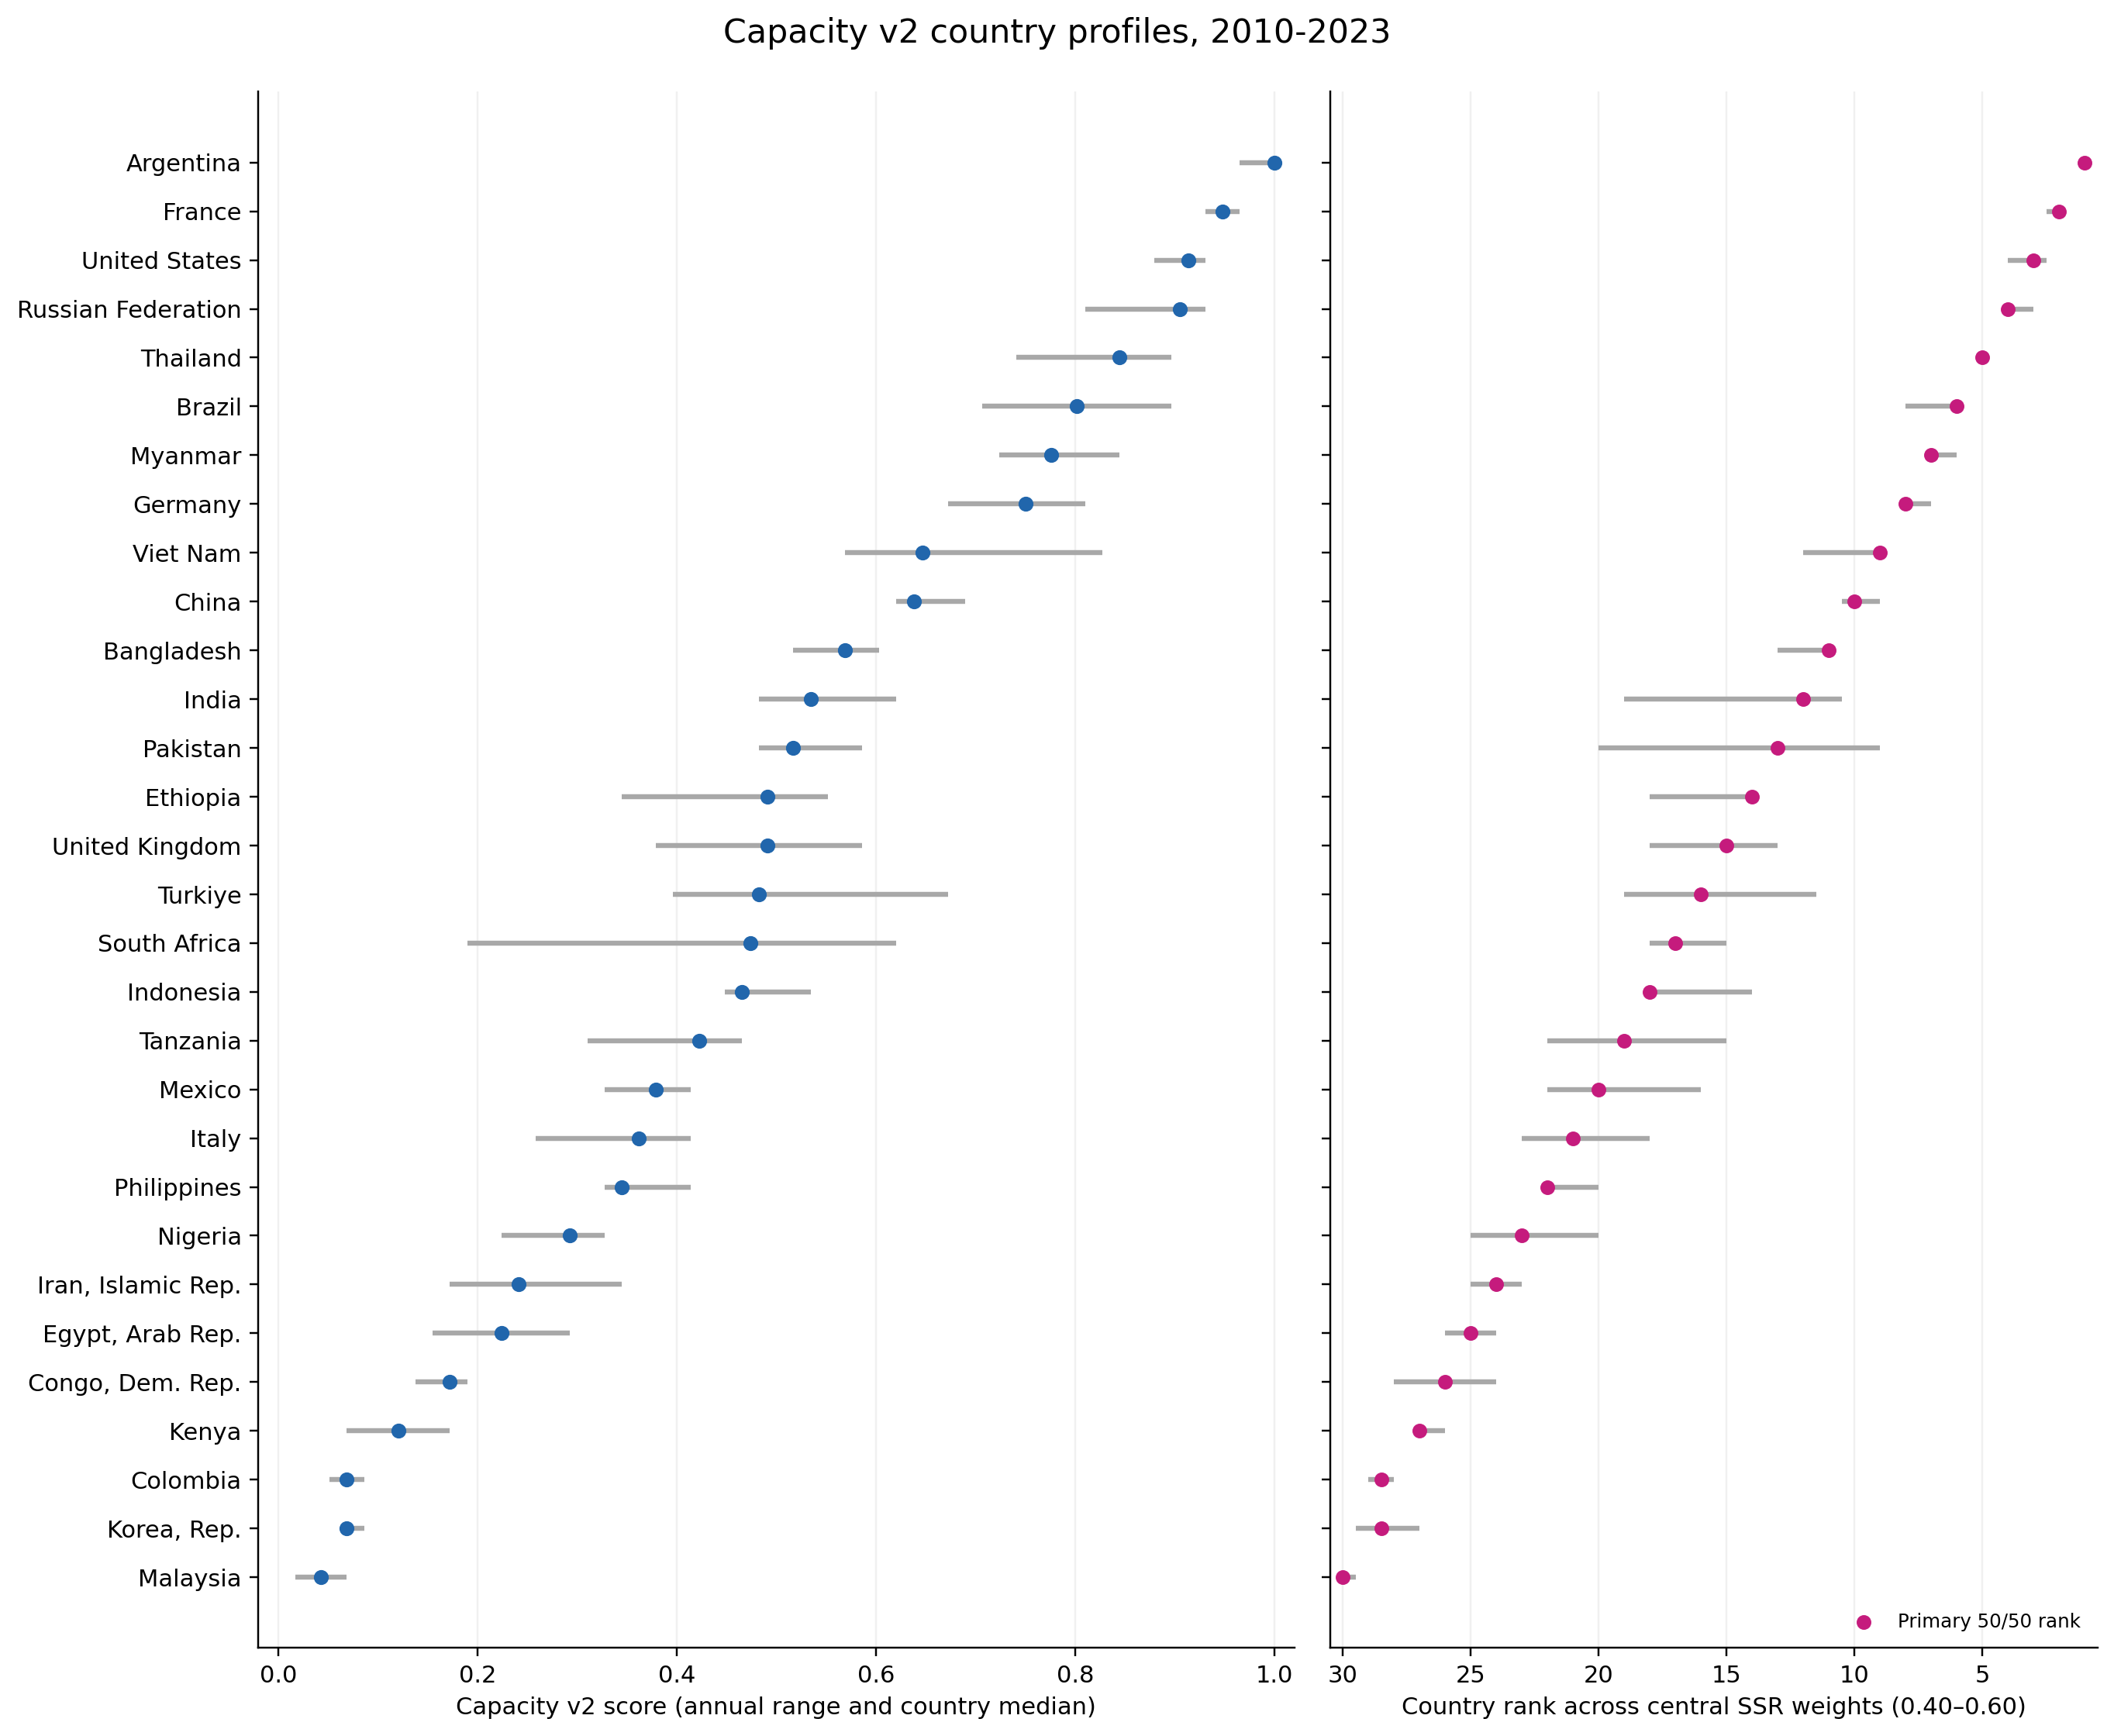
\includegraphics[width=0.97\textwidth]{../figures/capacity_profile.png}
\caption{Country capacity profiles. The primary ordering uses each country's median 50/50 score. Intervals show annual score variation and rank ranges under central weights; they are sensitivity summaries, not sampling confidence intervals.}
\label{fig:capacity}
\end{figure}

Two of the four original category hypotheses survive, and two are contradicted. This is informative rather than a failure to be optimized away. The old taxonomy combines production power, trade resilience, economic capacity, and hunger outcomes. v2 intentionally measures less. Category labels are therefore retained as expert comparison groups, not treated as ground truth.

\subsection{Country structure is visible but partly outlier-driven}

Silhouette width selects $k=4$ (0.514 versus 0.447 at $k=2$ and 0.473 at $k=3$). The within-country year-resampling median ARI is 0.899, exceeding the prespecified 0.60 display gate. The resulting sizes are 2, 21, 6, and 1 countries.

The small clusters matter for interpretation. Malaysia forms a singleton with unusually high fertilizer intensity in this sample, while Argentina and Russia form a two-country group dominated by high arable land per person. A six-country group---Congo, Tanzania, Ethiopia, Kenya, Myanmar, and Nigeria---is separated mainly by low electricity access and a more rural/agricultural profile. The remaining 21 countries form a broad mixed cluster.

Accordingly, Figure~\ref{fig:clusters} is a profile map, not evidence that the world contains four stable food-system types. The bootstrap fixes both the country sample and $k=4$; it shows that the same extreme profiles persist when years are resampled, not that the taxonomy generalizes to other countries or samples.

\begin{figure}[H]
\centering
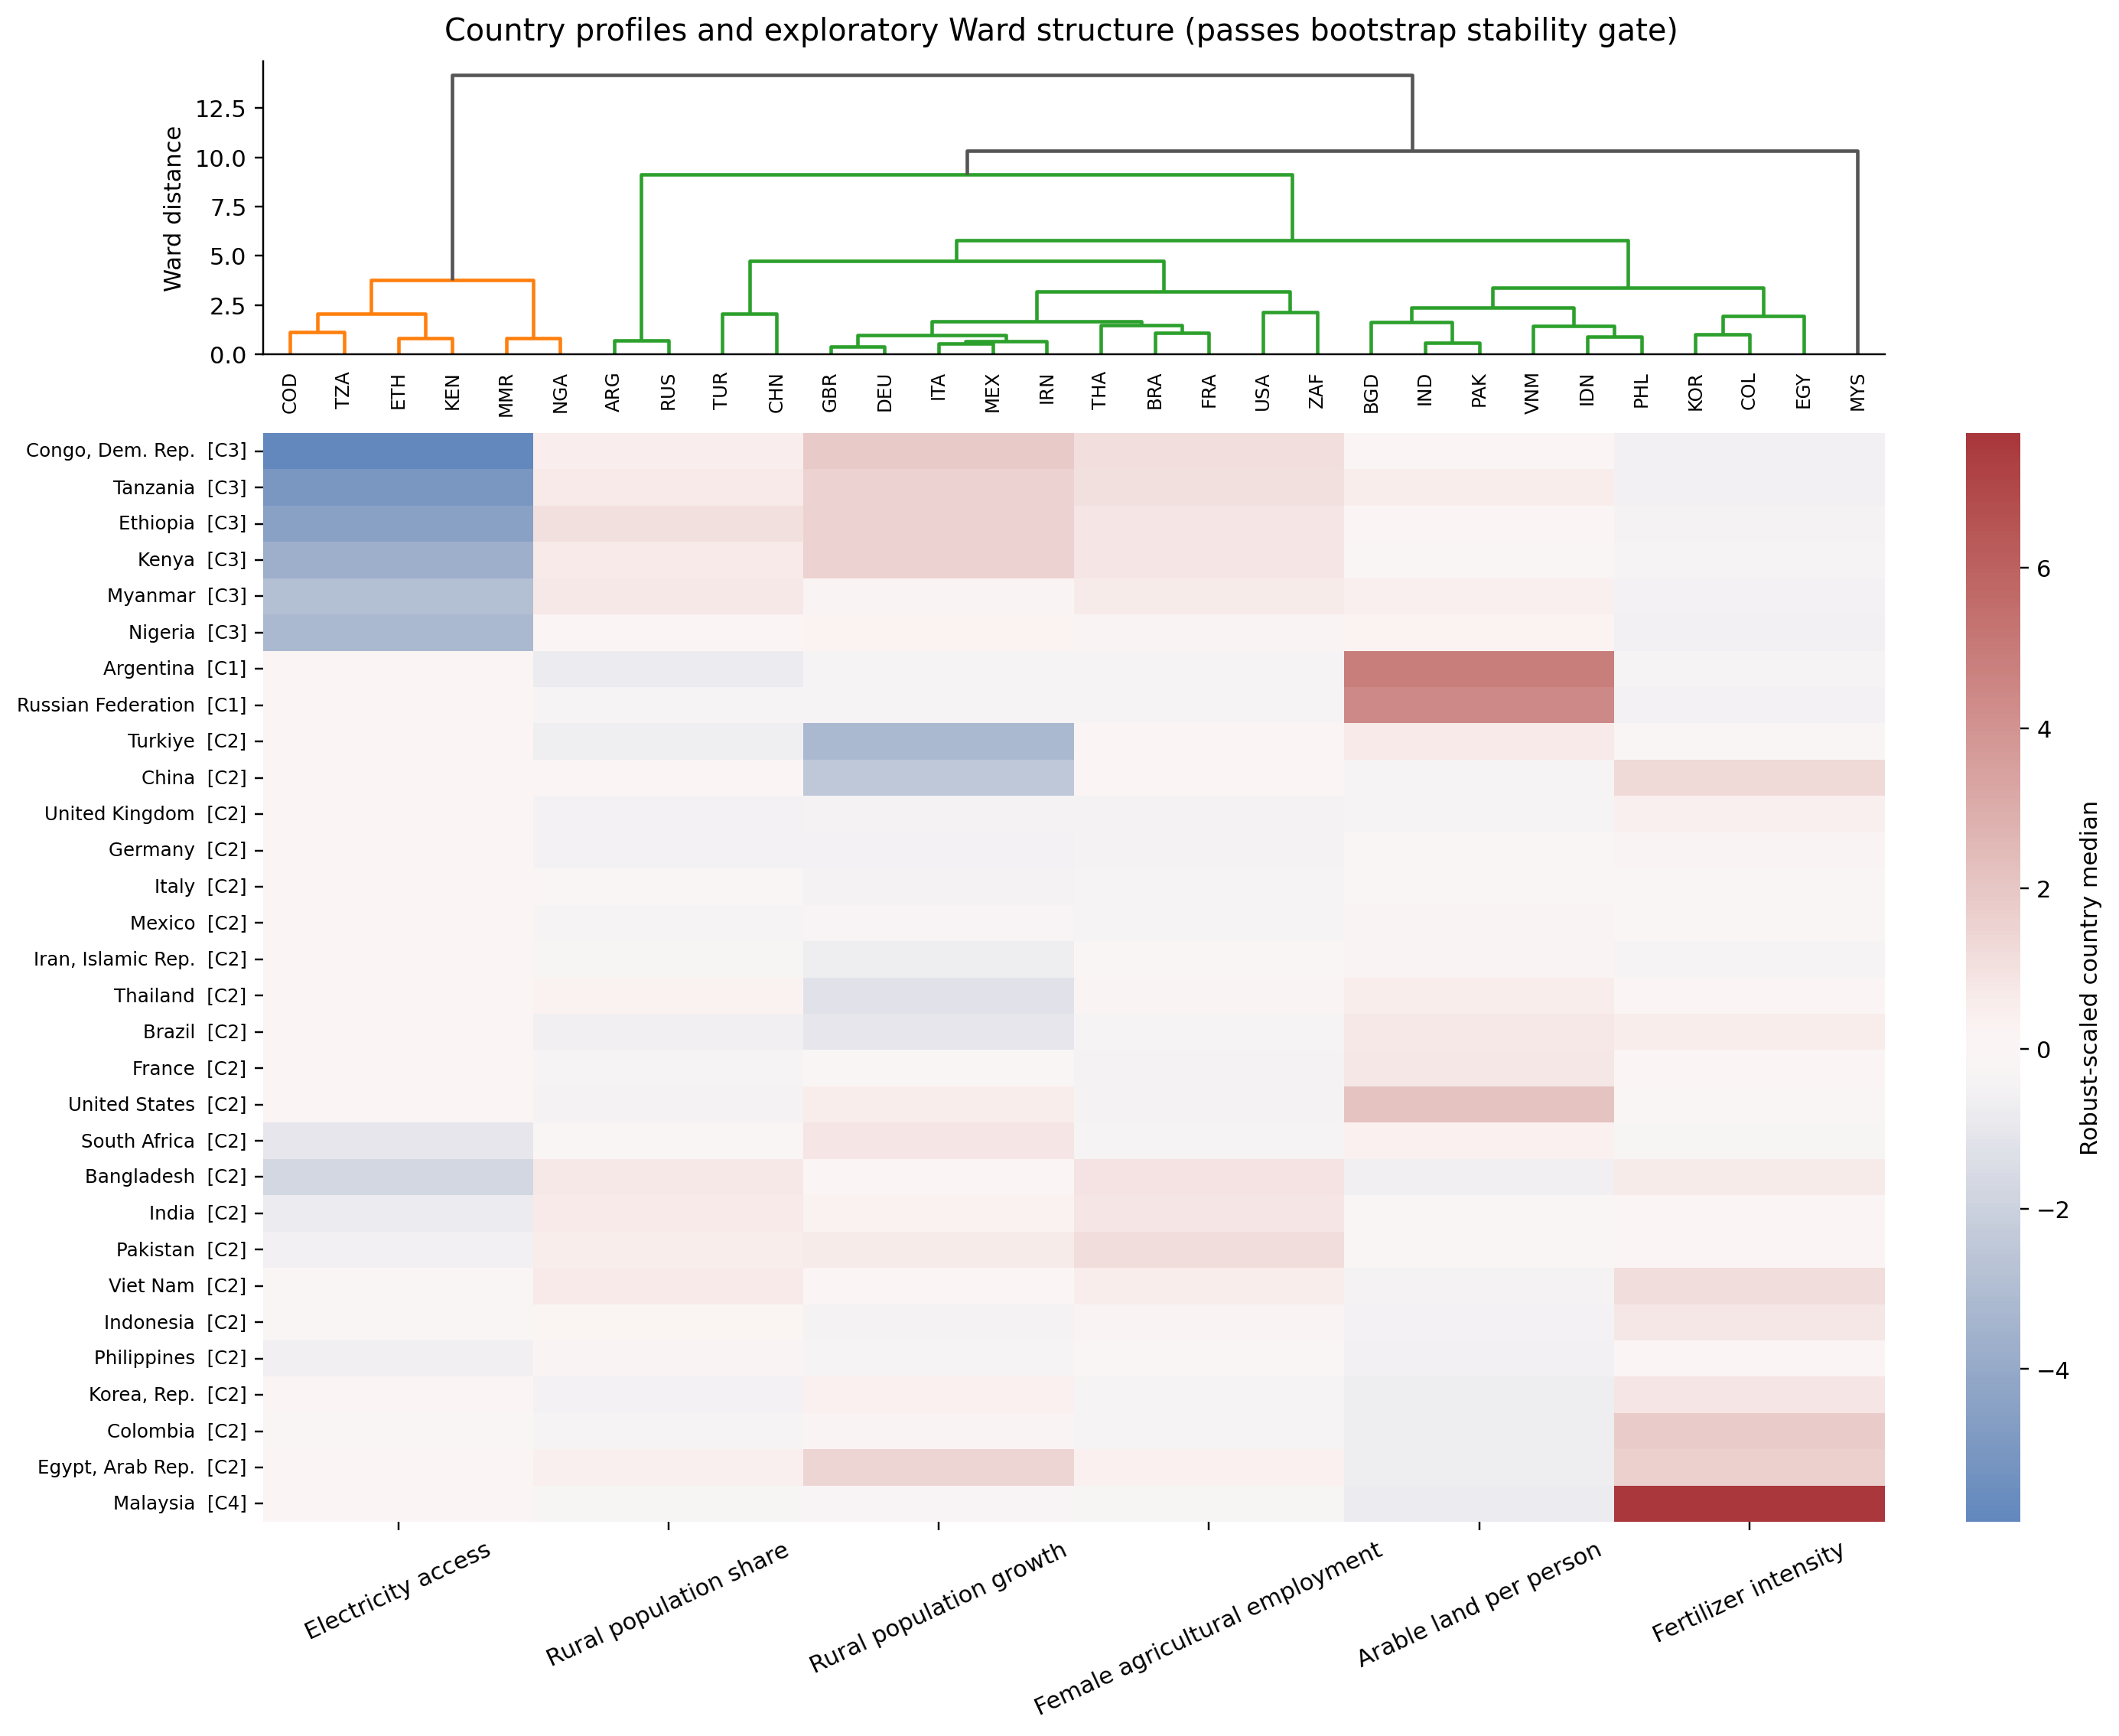
\includegraphics[width=0.98\textwidth]{../figures/country_structure.png}
\caption{Exploratory Ward clustering of robust-scaled 2010--2021 country medians. The heatmap exposes the extreme profiles that create the small clusters; Legacy categories are overlays rather than labels used to fit the clustering.}
\label{fig:clusters}
\end{figure}

\subsection{Models capture association, not dependable forecasting}

Table~\ref{tab:models} gives pooled out-of-fold results. OLS produces a moderate rank correlation (0.614) but negative $R^2$ and worse RMSE than the constant reference; 28 of 360 OLS predictions also exceed the score's upper bound of 1. The linear model therefore orders many held-out observations reasonably while calibrating the score poorly.

The shallow random forest improves pooled MAE by 16.7\% and RMSE by 17.5\% relative to the constant benchmark, reaching pooled $R^2=0.319$. This aggregate gain is not uniform: only three of five folds improve MAE, only two have positive $R^2$, and fold Spearman correlations range from 0.037 to 0.858. The result supports limited out-of-country structure in the constructed index, not a strong prediction or forecasting claim.

\begin{table}[H]
\centering
\caption{Country-grouped model validation and attribution audit.}
\label{tab:models}
\small
\begin{tabularx}{\textwidth}{L{2.45cm} L{1.25cm} L{1.25cm} L{1.10cm} L{1.20cm} Y}
\toprule
Model/audit & MAE & RMSE & $R^2$ & \rhoS & Fold and interpretation diagnostic \\
\midrule
Constant 0.50 & 0.230 & 0.277 & 0.000 & \NA & Common reference; no estimated model \\
OLS & 0.225 & 0.308 & $-0.231$ & 0.614 & 3/5 positive-$R^2$ folds; fold $R^2$ $[-2.72,0.63]$; 28/360 predictions $>1$ \\
Shallow random forest & 0.192 & 0.229 & 0.319 & 0.562 & 2/5 positive-$R^2$ folds; 3/5 folds beat baseline MAE; fold $R^2$ $[-0.63,0.74]$ \\
\midrule
OLS sign audit & \multicolumn{4}{l}{All six coefficient signs repeat in 5/5 grouped folds} & Sign agreement does not repair weak out-of-country calibration \\
RF importance audit & \multicolumn{4}{l}{Arable land/person: mean held-out $\Delta$MAE 0.070; positive in 5/5 folds} & Only feature with consistently positive incremental held-out importance \\
RF rank audit & \multicolumn{4}{l}{Median pairwise fold importance-rank \rhoS=0.486} & ``Top five of six'' is too permissive to establish broad feature stability \\
\bottomrule
\end{tabularx}
\end{table}

The full-panel OLS associations, expressed per predictor standard deviation, are shown in Figure~\ref{fig:ols}. Arable land per person has the largest positive coefficient ($+0.179$, 95\% country-clustered interval $[0.107,0.251]$). Electricity access ($+0.119$) and rural population share ($+0.154$) are also positive conditional associations, while fertilizer intensity is negative ($-0.061$). Rural population growth and female agricultural employment have intervals crossing zero.

These are not intervention effects. For example, the positive conditional rural-share coefficient should not be read as ``increasing rural population improves capacity,'' and the negative fertilizer coefficient should not be read as a recommendation to reduce inputs. Both may reflect country mix, nonlinearities, correlated structure, and the target's construction.

\begin{figure}[H]
\centering
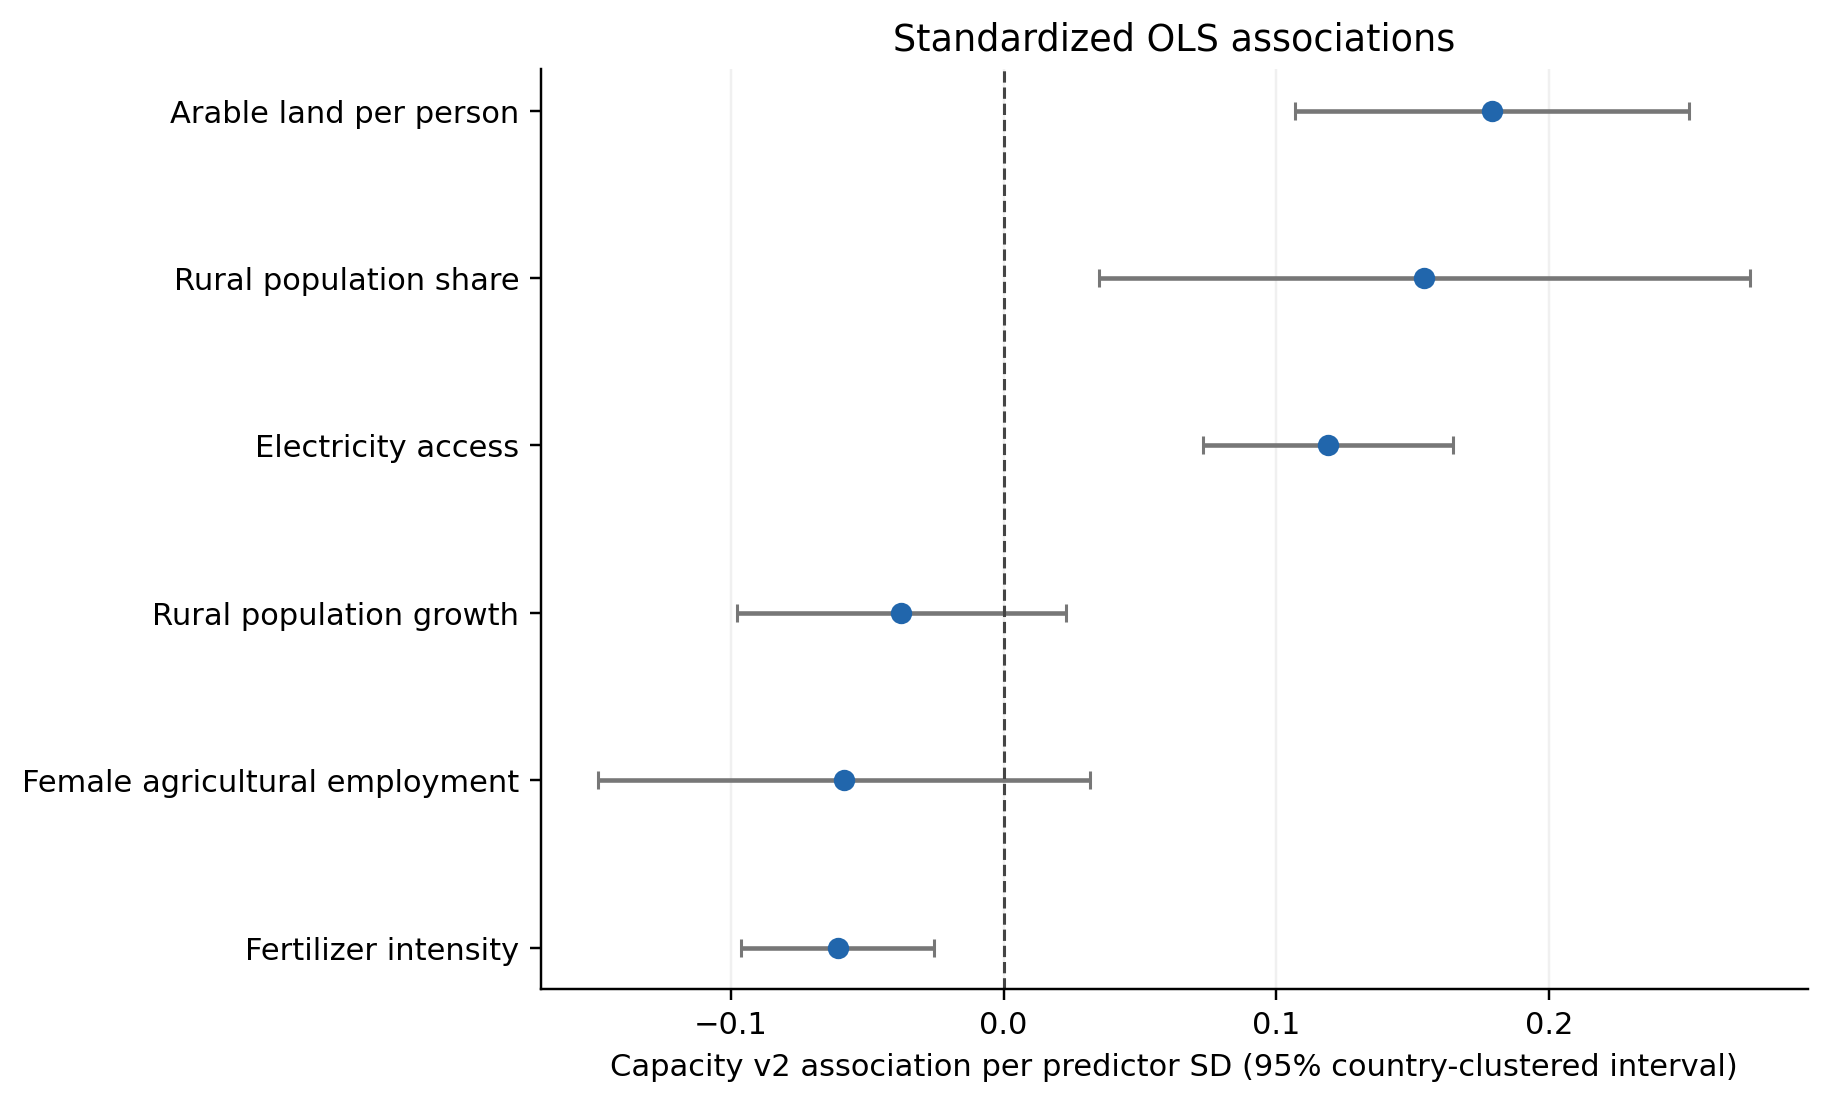
\includegraphics[width=0.90\textwidth]{../figures/linear_coefficients.png}
\caption{OLS conditional associations with Capacity Score v2. Predictors are standardized; intervals use country-clustered standard errors. The figure is descriptive and does not identify causal effects.}
\label{fig:ols}
\end{figure}

The nonlinear explanation audit further narrows the claim. Arable land per person is the only feature with positive held-out permutation importance in every fold and clearly dominates the mean importance. Fertilizer, rural growth, rural share, female agricultural employment, and electricity contribute small, mixed, or sometimes negative incremental held-out value. A single cross-fitted SHAP summary is retained in Appendix~\ref{app:models} as an exploratory diagnostic; ICE, PDP, dependence galleries, and additional tree models were not run.

\subsection{External outcomes align weakly in the intended direction}

Capacity v2 has modest inverse country-rank associations with PoU and FIES (Table~\ref{tab:external}). The PoU lower- and upper-bound views both give \rhoS=-0.31 because moving $<2.5$ values between their bounds does not change the country-median ordering. This does not convert censored values into exact observations. FIES gives \rhoS=-0.27 on 27 countries with exact published values; China, India, and T\"urkiye have no exact values in the aligned FIES extraction.

\begin{table}[H]
\centering
\caption{External construct alignment of country-median Capacity Score v2. Correlations are descriptive.}
\label{tab:external}
\small
\begin{tabularx}{\textwidth}{L{2.45cm} L{1.30cm} L{1.85cm} L{1.55cm} Y}
\toprule
Outcome view & $N$ & Aligned exact/usable rows & \rhoS & Interpretation boundary \\
\midrule
PoU lower bound & 30 & 420; 137 left-censored & $-0.31$ & $<2.5$ contributes 0 only as a lower bound \\
PoU upper bound & 30 & 420; 137 left-censored & $-0.31$ & $<2.5$ contributes 2.5 only as an upper bound \\
FIES exact & 27 & 218 exact; 202 excluded & $-0.27$ & Published exact three-year averages only; coverage ranges 3--9 periods per country \\
GHI 2025 edition & 24 & 24 sparse aligned points & $-0.33$ & Appendix sensitivity; same edition only; no interpolation \\
\bottomrule
\end{tabularx}
\end{table}

The negative signs are consistent with the intended interpretation: countries with stronger cereal capacity tend, on average, to rank lower on hunger and food-insecurity outcomes. The magnitudes are not strong enough to treat v2 as a validated measure of hunger or household food access. Capacity is one upstream national condition; PoU and FIES capture different constructs and are influenced by income, distribution, prices, conflict, policy, and many other mechanisms.

\section{Discussion}

\subsection{What the project now demonstrates}

The revised project demonstrates a coherent sequence of analytical decisions rather than a catalog of algorithms:

\begin{itemize}
  \item \textbf{Data provenance:} official API and catalog extracts are archived with definitions, dates, URLs, and hashes. Censoring, suppression, and absence remain semantically distinct.
  \item \textbf{Transparent index design:} the score has two readable components and a prespecified default weight. Complete sensitivity grids are shown instead of selecting a favorable weight after seeing outcomes.
  \item \textbf{Respectful treatment of expert judgment:} the original categories are preserved and tested. Contradictions are reported rather than interpreted as a need to force the data into the taxonomy.
  \item \textbf{Validation aligned to the unit of generalization:} countries, not country-year rows, define model folds. This prevents years from the same held-out country leaking into training.
  \item \textbf{Explanation with a failure condition:} OLS and one shallow forest are kept because they offer complementary conditional and nonlinear descriptions. Weak or unstable explanations are demoted rather than multiplied.
  \item \textbf{Negative evidence:} the earlier PoU forecasting gate failed against persistence and remains part of the record. The project is consequently framed as index construction and attribution, not forecasting.
\end{itemize}

This sequence is more valuable than a high in-sample score. Because the target is constructed from ranks, extremely high fit could simply indicate that predictors reconstruct the chosen index. The present grouped results are less flattering but more informative: the forest captures some transferable structure, yet performance varies sharply with which countries are held out.

\subsection{Why the removed analyses were redundant}

The earlier report used t-SNE, multiple GLM families, Random Forest, XGBoost, LightGBM, broad SHAP output, PDP, and many Category-specific ICE plots. That breadth created three problems. First, several models answered the same reconstruction question. Second, random row splits allowed the same countries to appear in training and test years. Third, large explanation galleries encouraged storytelling without testing whether feature importance persisted across held-out countries.

The revised report keeps one linear and one nonlinear model, one grouped validation design, and a compact stability audit. The SHAP beeswarm remains only because it summarizes the fitted forest's cross-fitted attributions; it is not a headline result. The Category ICE/PDP plots are removed because they condition on a fitted model of a constructed target, use small expert-defined groups, and add little beyond the direct category comparisons and the global association audit.

\section{Limitations}

\begin{enumerate}
  \item \textbf{Construct limitation.} v2 measures cereal supply/trade capacity, not multidimensional food security. It omits affordability, distribution, utilization, diet quality, shocks, and within-country inequality.
  \item \textbf{Related components.} Production contributes to both SSR and production per person. Equal weights improve transparency but do not prove equal construct importance.
  \item \textbf{Selected country scope.} The 30-country panel is a course-project sample conditioned on complete modern SSR coverage. Japan is absent from v2, and the sample is not representative of all countries.
  \item \textbf{Relative score.} Annual percentile ranks depend on the comparison set and do not provide an absolute capacity threshold.
  \item \textbf{Small effective sample for generalization.} Although the model panel has 360 rows, there are only 30 independent country groups. Five-fold results are correspondingly sensitive to the held-out country mix.
  \item \textbf{Clustering sensitivity.} The selected four-cluster cut contains a singleton and a two-country cluster. Within-country year bootstrap stability does not test stability to adding or removing countries.
  \item \textbf{Associational models.} OLS coefficients, permutation importance, and SHAP values describe model associations with a constructed target. They do not identify policy effects or causal mechanisms.
  \item \textbf{Outcome semantics.} PoU contains left-censored values, FIES is incomplete and suppressed for some countries, and GHI is sparse. Country-median correlations discard temporal detail and remain descriptive.
  \item \textbf{Data vintage.} The reconstruction uses archived current releases, not real-time historical vintages. Later revisions by source organizations can change exact values.
  \item \textbf{Local protocol.} The analysis contract was fixed before execution and outputs were independently verified, but it was not externally preregistered.
\end{enumerate}

\section{Conclusion}

The project can now be explained in one sentence: \emph{it builds a transparent two-component cereal-capacity index, tests rather than forces expert assumptions, maps country profiles, and uses country-grouped models to identify cautious structural associations before checking whether the score aligns directionally with official hunger outcomes.}

The evidence supports retaining Capacity Score v2 as a descriptive case-study artifact. Its ranking is robust to central weights and normalization, but it is narrower than the Legacy taxonomy. Country structure is exploratory and partly driven by extremes. The random forest improves pooled out-of-country error, but fold heterogeneity rules out a strong forecasting claim. Arable land per person is the clearest repeated model attribution. PoU and FIES point in the expected direction but confirm that cereal capacity is not equivalent to food access or hunger.

This is a stronger portfolio narrative than the original algorithm-heavy report because every method now has a distinct role and boundary. The public repository excludes the original submission and sensitive provenance files. The owner confirms sole authorship, so CV descriptions may present it as an independently completed project; the later AI-assisted reconstruction is disclosed below.

\section*{Reproducibility, Data Availability, and Declarations}
\addcontentsline{toc}{section}{Reproducibility, Data Availability, and Declarations}

\textbf{Reproducibility.} The revised workspace preserves raw-source snapshots, processed panels, deterministic scripts, machine-readable result tables, manifests, and SHA-256 hashes. An independent result-package verifier passed 44 of 44 checks, including input/output hashes, row and country counts, grouped-fold separation, prohibited-method guards, and figure readability. The archived original R Markdown and PDF remain byte-identical to their preserved copies.

\textbf{Data availability.} The public repository provides the reusable reconstruction code, compact processed World Bank/FAOSTAT inputs, result tables, figures, and this report. Raw third-party workbooks and the original course submission are excluded. Source organizations make the underlying data available under their respective terms.

\textbf{Ethics and unit of analysis.} The analysis uses public country-level aggregate data and involves no human participants or personal data. Country-level results must not be interpreted as individual or household outcomes.

\textbf{Authorship and contributions.} This was a solo course project completed independently by the repository owner, who handled research framing, data collection and preprocessing, index design, modeling, interpretation, visualization, and reporting.

\textbf{AI-assisted reconstruction disclosure.} AI tools assisted with code review, reproducibility checks, and prose restructuring. Reported values come from saved scripts and verified artifacts; responsibility for the public release remains with the repository owner.

\textbf{Funding and conflicts of interest.} The available project record does not document external funding or a conflict of interest; no broader claim is made.

\clearpage
\begin{thebibliography}{99}
\small

\bibitem{worldbankapi}
World Bank. (n.d.). \textit{About the Indicators API documentation}. World Bank Data Help Desk. \url{https://datahelpdesk.worldbank.org/knowledgebase/articles/889392}

\bibitem{worldbankqueries}
World Bank. (n.d.). \textit{Indicator API queries}. World Bank Data Help Desk. \url{https://datahelpdesk.worldbank.org/knowledgebase/articles/898599-indicator-api-queries}

\bibitem{faohandbook}
Food and Agriculture Organization of the United Nations. (n.d.). \textit{Food balance sheet handbook: Concepts and definitions}. \url{https://www.fao.org/4/x9892e/X9892e04.htm}

\bibitem{faofbs}
Food and Agriculture Organization of the United Nations. (n.d.). \textit{Food Balances (2010--): Data catalog}. \url{https://data.fao.org/catalog/iso/2f264bb6-1238-459a-bf8b-0e2d0a16804a}

\bibitem{faohunger}
Food and Agriculture Organization of the United Nations. (n.d.). \textit{Measuring hunger and food insecurity}. \url{https://www.fao.org/measuring-hunger/en}

\bibitem{ghimethod}
Global Hunger Index. (2025). \textit{Methodology}. \url{https://www.globalhungerindex.org/methodology.html}

\bibitem{ward1963}
Ward, J. H., Jr. (1963). Hierarchical grouping to optimize an objective function. \textit{Journal of the American Statistical Association, 58}(301), 236--244. \url{https://doi.org/10.1080/01621459.1963.10500845}

\bibitem{rousseeuw1987}
Rousseeuw, P. J. (1987). Silhouettes: A graphical aid to the interpretation and validation of cluster analysis. \textit{Journal of Computational and Applied Mathematics, 20}, 53--65. \url{https://doi.org/10.1016/0377-0427(87)90125-7}

\bibitem{hubertarabie1985}
Hubert, L., \& Arabie, P. (1985). Comparing partitions. \textit{Journal of Classification, 2}, 193--218. \url{https://doi.org/10.1007/BF01908075}

\bibitem{breiman2001}
Breiman, L. (2001). Random forests. \textit{Machine Learning, 45}, 5--32. \url{https://doi.org/10.1023/A:1010933404324}

\bibitem{lundberglee2017}
Lundberg, S. M., \& Lee, S.-I. (2017). A unified approach to interpreting model predictions. In \textit{Advances in Neural Information Processing Systems 30}. \url{https://proceedings.neurips.cc/paper/2017/hash/8a20a8621978632d76c43dfd28b67767-Abstract.html}

\end{thebibliography}

\clearpage
\appendix
\section{Legacy Weight-Search Reproduction}
\label{app:legacy}

The historical audit evaluated all 5,151 one-percentage-point triples. Of these, 1,380 satisfy the four Legacy category constraints. The minimum original TV diagnostic is 0.245161, shared by three weight triples. Under the original R \texttt{expand.grid} traversal, 0.19/0.15/0.66 is the first tied minimum (row 1,430), so the published result is exactly reproducible but not unique. The reconstructed fixed score matches the archived panel to a maximum absolute difference of $8.33\times10^{-16}$.

\begin{figure}[H]
\centering
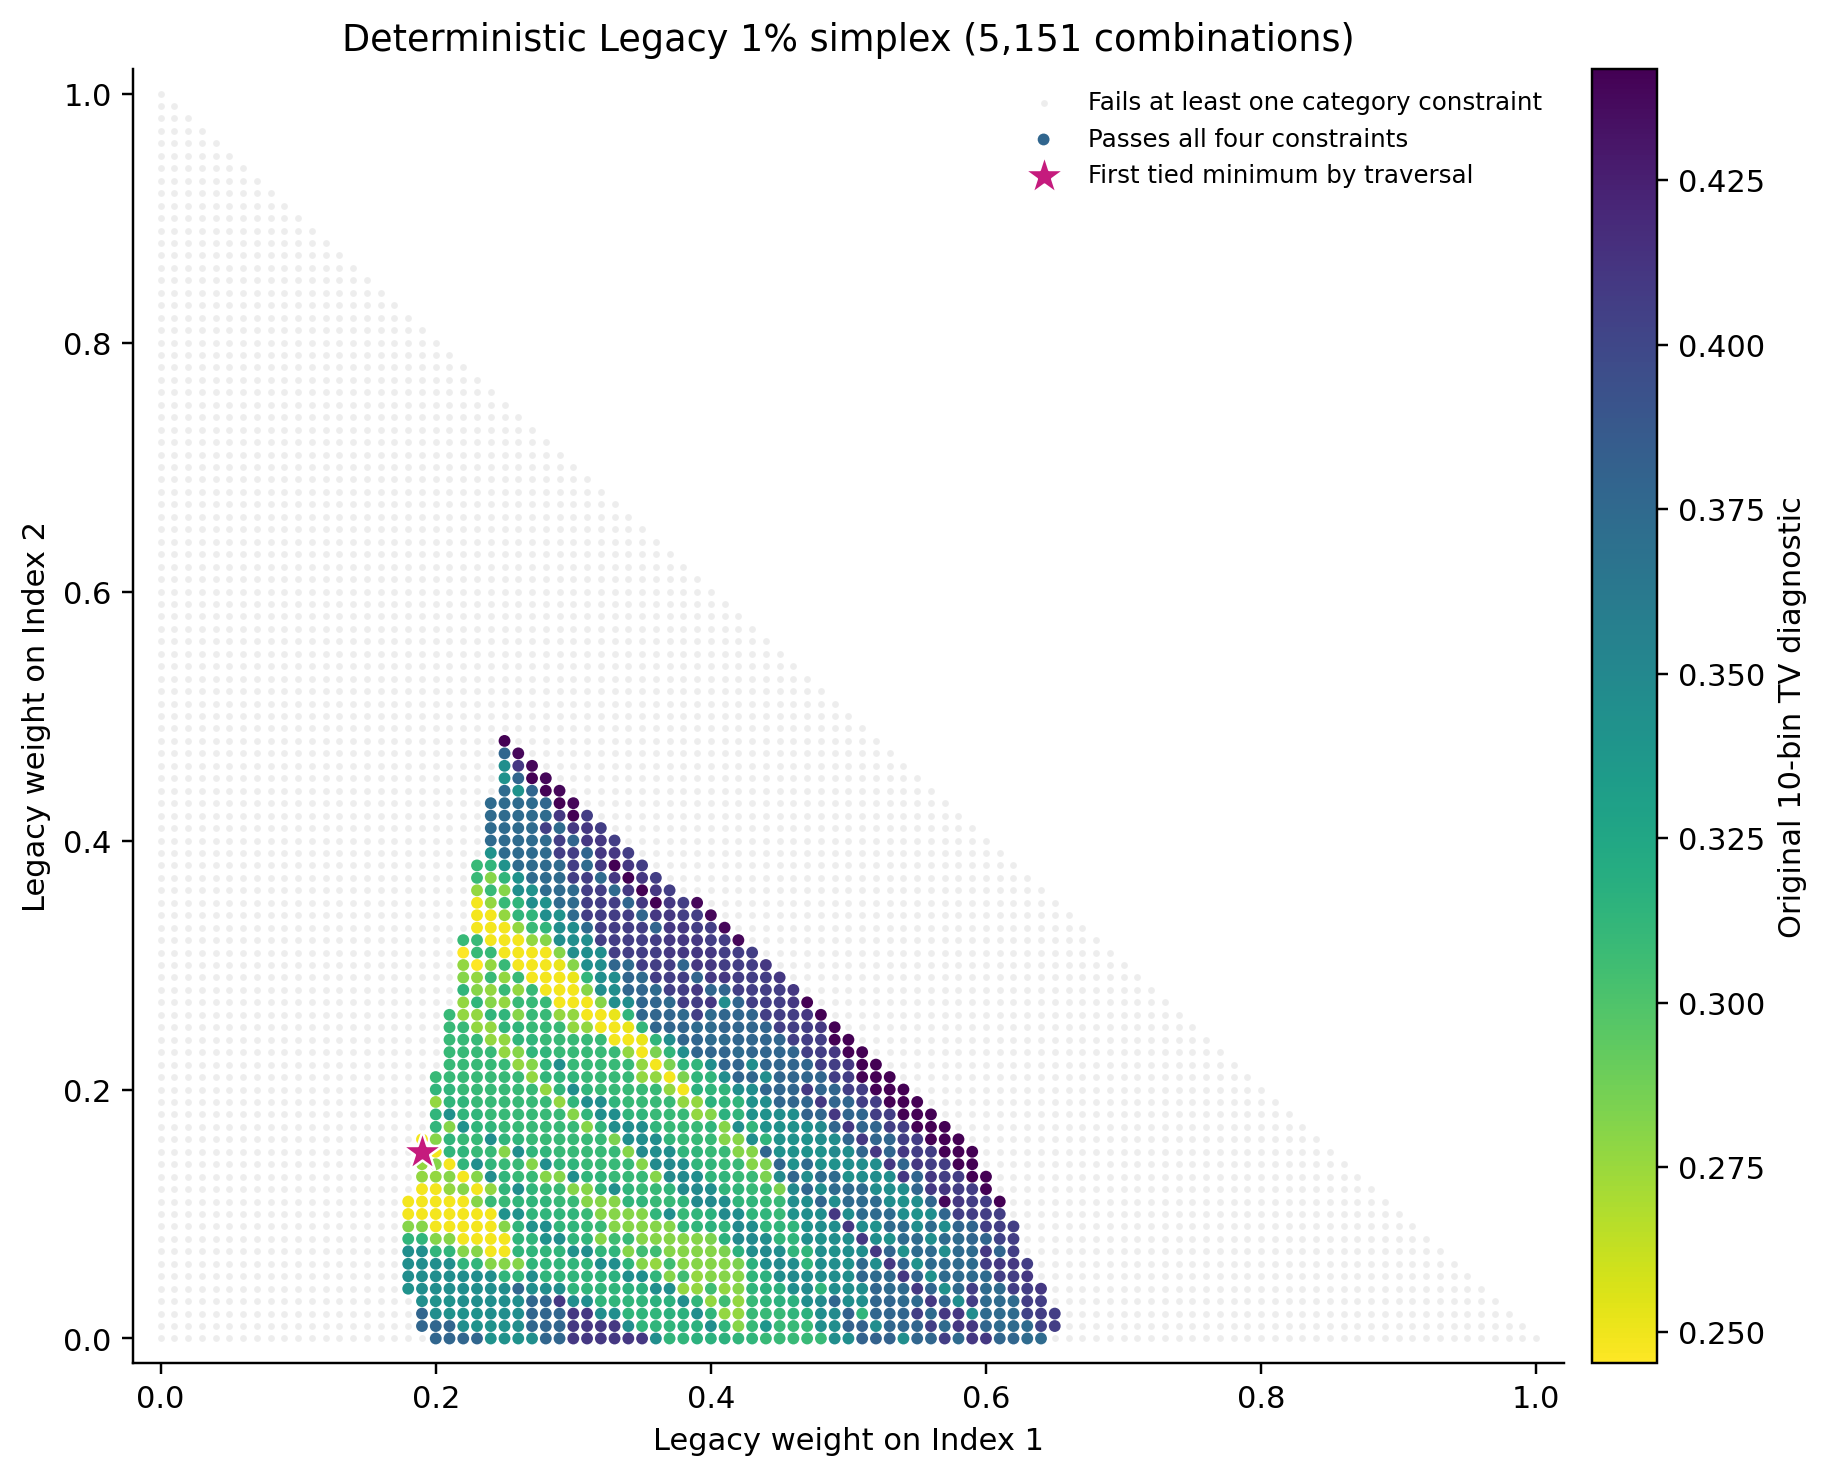
\includegraphics[width=0.96\textwidth]{../figures/legacy_simplex_appendix.png}
\caption{Complete deterministic Legacy simplex. The highlighted solution is the first of three tied minimum-TV solutions among category-valid weights.}
\end{figure}

This audit preserves the historical method without restoring its GHI interpolation or treating its category constraints as external validation.

\section{Clustering Diagnostics}
\label{app:clusters}

Silhouette scores were 0.447 ($k=2$), 0.473 ($k=3$), 0.514 ($k=4$), 0.335 ($k=5$), and 0.355 ($k=6$). The 500 within-country year-resampling ARIs had median 0.899 and 5th/95th percentiles 0.671/1.000. Cluster membership was:

\begin{itemize}
  \item Cluster 1 (2): Argentina, Russian Federation;
  \item Cluster 2 (21): Bangladesh, Brazil, China, Colombia, Germany, Egypt, France, United Kingdom, Indonesia, India, Iran, Italy, Korea, Mexico, Pakistan, Philippines, Thailand, T\"urkiye, United States, Viet Nam, South Africa;
  \item Cluster 3 (6): Congo (Dem. Rep.), Ethiopia, Kenya, Myanmar, Nigeria, Tanzania;
  \item Cluster 4 (1): Malaysia.
\end{itemize}

The extreme robust-scaled values---Malaysia fertilizer intensity (7.68) and Argentina/Russia arable land (4.91/4.39)---explain why the main text avoids substantive cluster names. The bootstrap resamples years but never removes these countries.

\section{Fold-Level Model and Explanation Diagnostics}
\label{app:models}

\begin{table}[H]
\centering
\caption{Fold-level validation on six held-out countries per fold.}
\small
\begin{tabular}{crrrr}
\toprule
Fold & Model & MAE & $R^2$ & Spearman \\
\midrule
1 & OLS & 0.160 & 0.634 & 0.835 \\
1 & RF  & 0.154 & 0.694 & 0.858 \\
2 & OLS & 0.230 & $-1.094$ & 0.726 \\
2 & RF  & 0.220 & $-0.152$ & 0.723 \\
3 & OLS & 0.131 & 0.315 & 0.549 \\
3 & RF  & 0.187 & $-0.065$ & 0.037 \\
4 & OLS & 0.201 & 0.145 & 0.253 \\
4 & RF  & 0.104 & 0.740 & 0.851 \\
5 & OLS & 0.404 & $-2.720$ & 0.729 \\
5 & RF  & 0.293 & $-0.627$ & 0.686 \\
\bottomrule
\end{tabular}
\end{table}

Arable land per person has mean held-out permutation $\Delta$MAE 0.0698 and is positive in all five folds. The remaining mean increases are 0.0069 (female agricultural employment), 0.0053 (fertilizer), 0.0010 (rural population growth), $-0.0002$ (rural share), and $-0.0025$ (electricity), with mixed fold signs or small magnitudes. Correlated predictors can share information, so near-zero incremental importance does not prove no association; it does prevent a claim of robust standalone importance.

\begin{figure}[H]
\centering
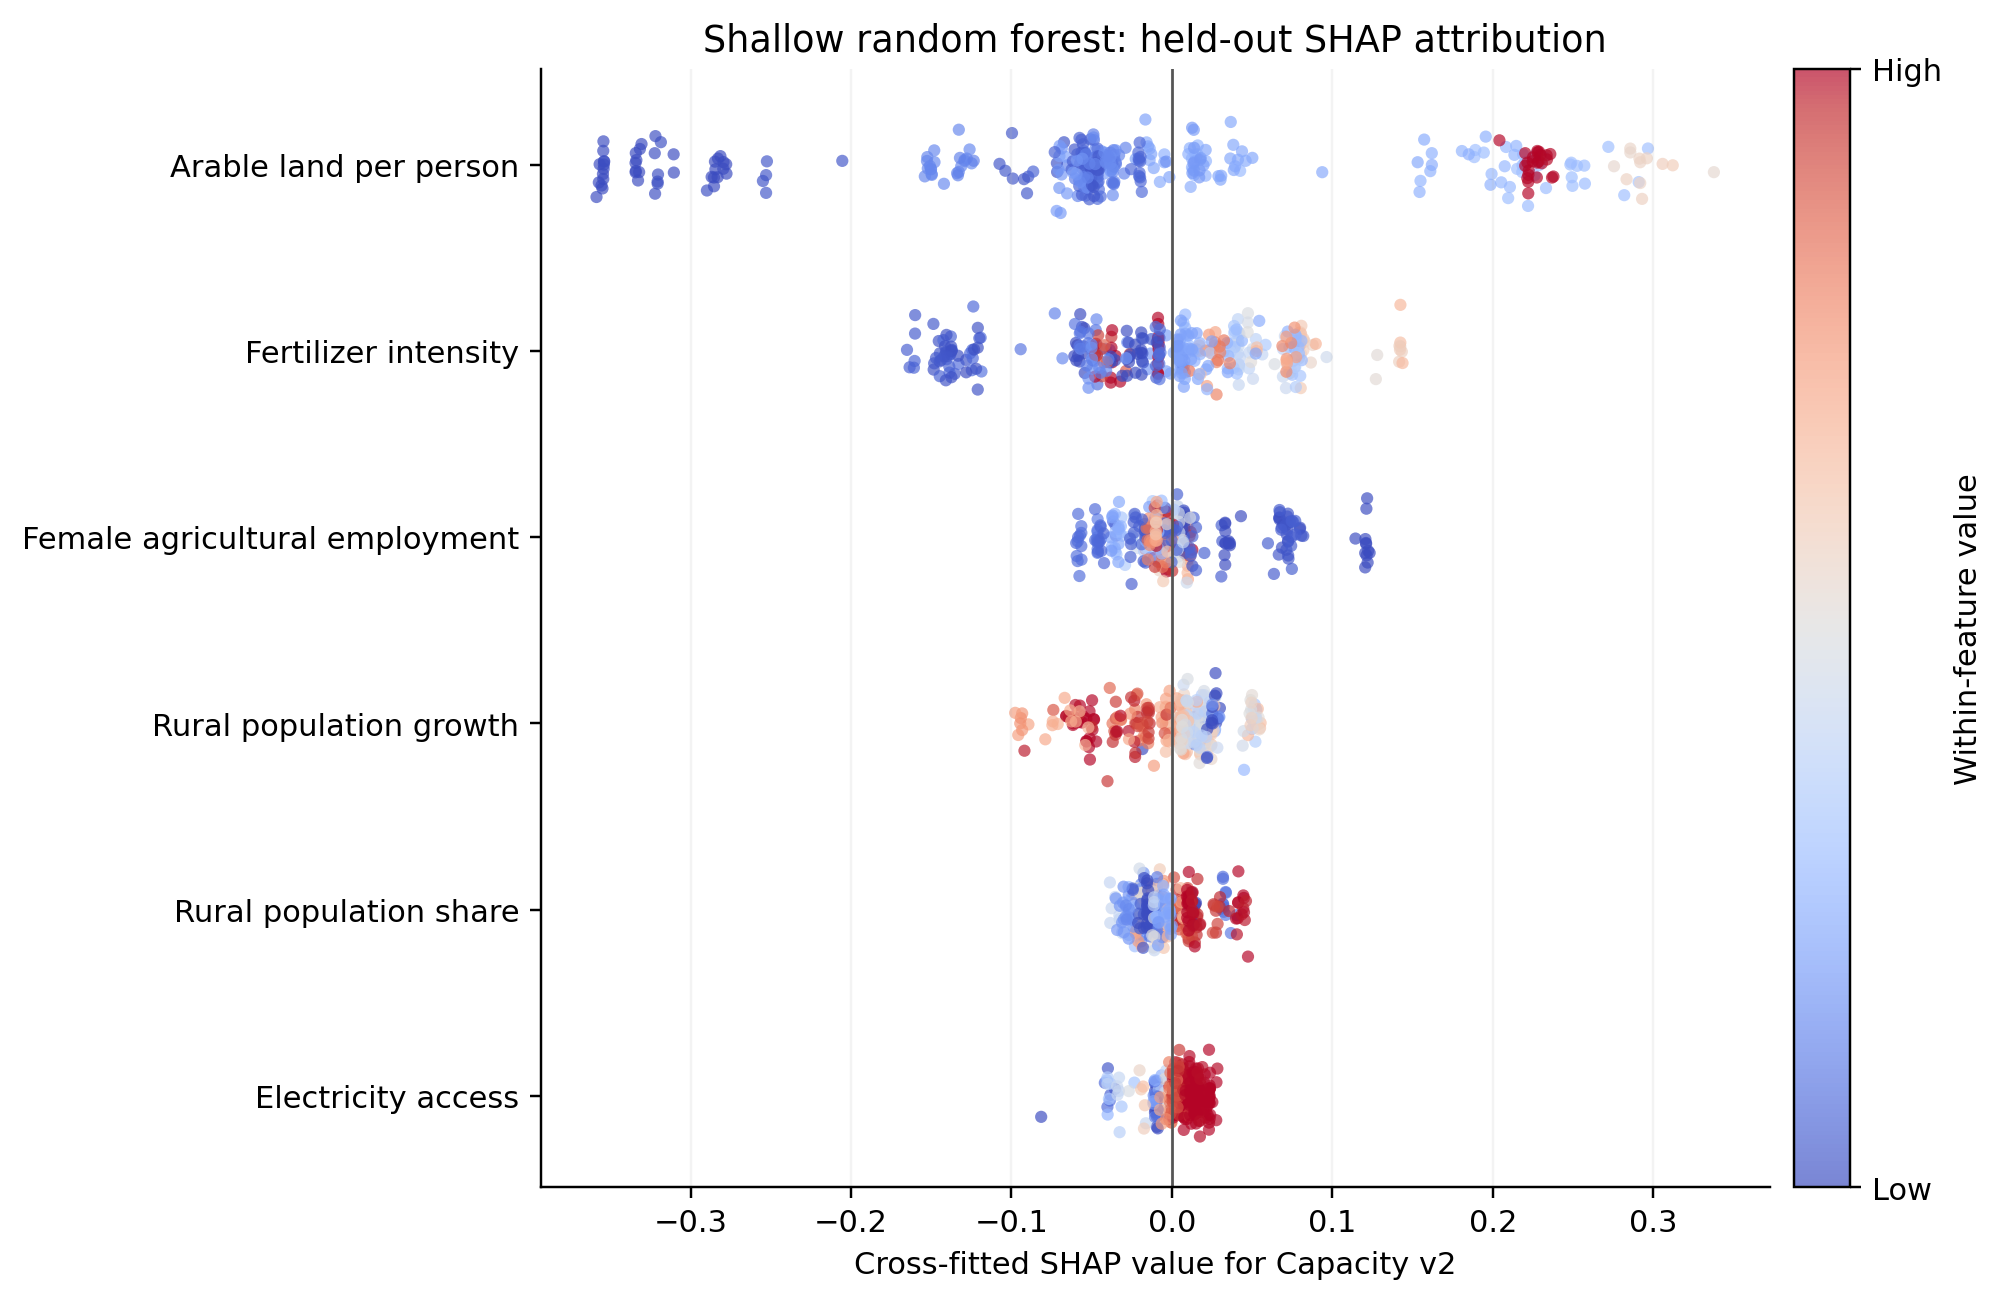
\includegraphics[width=0.92\textwidth]{../figures/rf_shap_beeswarm_appendix.png}
\caption{Cross-fitted random-forest SHAP summary, retained only as an exploratory appendix diagnostic. Direction-consistent color patterns do not override weak or inconsistent held-out permutation importance.}
\end{figure}

\section{Sparse Outcome and Negative Forecast Sensitivities}

The same-edition GHI check uses only 24 countries and one aligned reference point per country in the v2 window; its rank association is approximately $-0.33$. It is too sparse for a main validation claim and is not interpolated.

The earlier forward PoU gate used non-overlapping three-year target periods and a held-out 2019 test period. Persistence MAE was 0.894. Ridge variants produced test MAE 1.425--1.549, and interval-censored Tobit variants produced MAE 1.452--1.457. Capacity coefficients had the expected negative sign, but every model underperformed persistence. No tree model or SHAP analysis was permitted for that forecasting target after the gate failed.

\section{Artifact Verification}

The final result package records 30 countries, 420 index rows, 360 model rows, 500 clustering bootstraps, 2,160 cross-fitted base-feature SHAP rows, zero train/test country overlap, and no missing predictions. The independent verification passed all 44 checks. Guardrails confirm that target ingredients and outcomes were excluded from predictors; only OLS and the fixed shallow random forest were run; no t-SNE, XGBoost, LightGBM, GLM sweep, ICE, PDP, forecast, or causal-identification analysis was added to the revised core.

\end{document}
